\chapter{Introduction}

\emph{``There are only two hard things in Computer Science: cache invalidation and naming things.''} \vspace{-1cm}
\begin{flushright}-- Phil Karlton\end{flushright}

Web applications are becoming more and more dynamic with more personalized content that often requires complex data queries or computations based on large amounts of data. These computations can become a performance bottleneck in the application, which leads to slow response times and poor user experience for the users.

The performance can often be optimized by profiling and analyzing the code behind the computation, but this often not the easiest solution and in some cases the complexity or amount of data used makes it difficult achieve a satisfactory performance. Caching is a popular solution for improving the performance and scalability in these cases since it allows for a simple, scalable and generic way of addressing bottlenecks in the web applications.

Although it sounds like a silver bullet it also places a burden on the programmer that must locate and update the cached values while preserving consistency guarantees. This challenge is for example seen in an outage of the whole Facebook system:

\begin{quote}
  The intent of the automated system is to check for configuration values that are invalid in the cache and replace them with updated values from the persistent store. This works well for a transient problem with the cache, but it doesn’t work when the persistent store is invalid.

 Today we made a change to the persistent copy of a configuration value that was interpreted as invalid. This meant that every single client saw the invalid value and attempted to fix it. Because the fix involves making a query to a cluster of databases, that cluster was quickly overwhelmed by hundreds of thousands of queries a second.
\begin{flushright}Robert Johnson~\cite{facebook_outage}\end{flushright}
\end{quote}

This example shows how critical the caching system can be and the importance of correctness.

This thesis will address this issue by researching the latest caching technique proposed in research and used in practice and contribute with a design and implementation of a caching system in the Python programming language.

\section{Problem}
\label{sec:problem}

Most of the existing caching solutions are based on a pull based caching strategy, where the computation runs and the cached value is stored when the client requests the cached value. After the result has been computed and cached, the client will be presented with the cached value until it has been invalidated.

The pull based caching strategy has the advantage that we only have to cache content that is being used, but it also means that the first time a client asks for the value, it has to wait for the computation to finish. This is not optimal with relation to user experience since the user has to wait in order to be presented with the requested content. To solve this problem we have to precompute the cached values such that the user is presented with content as soon as it is requested.

Besides the performance problem on the initial request, existing caching solutions leaves responsibility for the programmers to maintain the cache in order ensure consistency and an appropriate level of freshness.

These problems with existing caching solutions, presents two major challenges:

\textbf{Cache Management}

The first challenge related to cache management is faced in any caching system, where the programmer has to manage the caching system by naming the cached value and keeping them up to date such that the users are not presented with unexpected content.

One particular challenge within cache management is \emph{cache invalidation} that relies on the programmer correctly identifying every underlying data that affects the given cached value. The programmer then has to declare a way for the cached value to be invalidated when any of the underlying data changes. This analysis is difficult since it require global reasoning about how the underlying data changes in the web application and which computations are cached. Furthermore if the computation behind the cached value is altered to depend on new underlying data, the cache invalidation also has to change, making the cache prone to errors if the latter is forgotten.

We discuss this more in chapter~\ref{chapter:caching} and~\ref{chapter:invalidation}.

\textbf{Data Update Propagation}

The second challenge is related to the task of efficiently keeping the cached values fresh while ensuring the consistency between the cache and the storage system. This challenge will be addressed in chapter~\ref{chapter:data-update-propagation}.

% section problem end

\section{Requirements}
\label{sec:requirements}

The final solution addressing the problems described, will be designed with the following non-functional requirements:

\textbf{Software design:} Must be designed to be maintainable such that the programmer that uses the caching system understands how it works from using it and has the ability to extend it. The design of the system should also be flexible to support multiple storage systems and caches.

\textbf{Adaptability:} Should be convenient and easy to adapt into existing systems. Furthermore the usage of the system should be easy to understand.

\textbf{Efficiency:} Should be efficient with relation to performance such that it does not make existing operations of the systems significantly slower. It should also be efficient with relation to the system load such that it does not use more computational power than necessary to achieve the goal of the system.

\textbf{Scalability:} Should be designed for scalability in the sense that the design should still be efficient for large amount of data and correct when the web application is scaled horizontally.

\textbf{Fault-Tolerance:} Should be designed with considerations on reliability, integrity and maintainability.

% section requirements end

\section{Context}
\label{sec:context}

The problem and requirements are based on a running web applications - the Peergrade.io-platform to ensure that the system is also designed, implemented and tested to be used in practice.

The problem description and requirements of the system is based on a practical problem experienced by a running web application - the Peergrade.io-platform. Throughout the thesis the system has been integrated and tested on the web application to ensure the system is designed and implemented with a practical perspective. Peergrade.io is a platform for facilitating peer-evaluation in university and high school courses. Currently the platforms serves multiple institutions and thousands of students.

\subsection{Peergrade.io Platform}
\label{subsec:the-peergrade-io-platform}

Universities and single teachers are able to sign up their courses to use Peergrade.io for facilitating peer-evaluation, where the students are able to grade and/or give each other feedback on their assignments. When a teacher has registered a course to use Peergrade.io, the teacher is able to create assignments. Beside the description of what the assignment is about, the teacher also sets deadlines for handing in and for the grading, and creates structured forms for the students to fill out with grades and text feedback.

When an assignment is open, the student is able to upload their hand-in for the assignment. After the deadline for handing in is reached, the Peergrade.io platform will automatically distribute hand-ins for students to answer feedback questions and give grades. When the deadline for grading is reached, the feedback and grades are made available to the author of the hand-in, and the authors are able to indicate give indicate the helpfulness of the feedback by giving a constructive score for the feedback or mark the feedback as inappropriate. After this step, the assignment is considered completed for the student. Figure~\ref{fig:student-screenshot} shows a screenshot of the Peergrade.io platform from the student's perspective.

\begin{figure*}[ht!]
  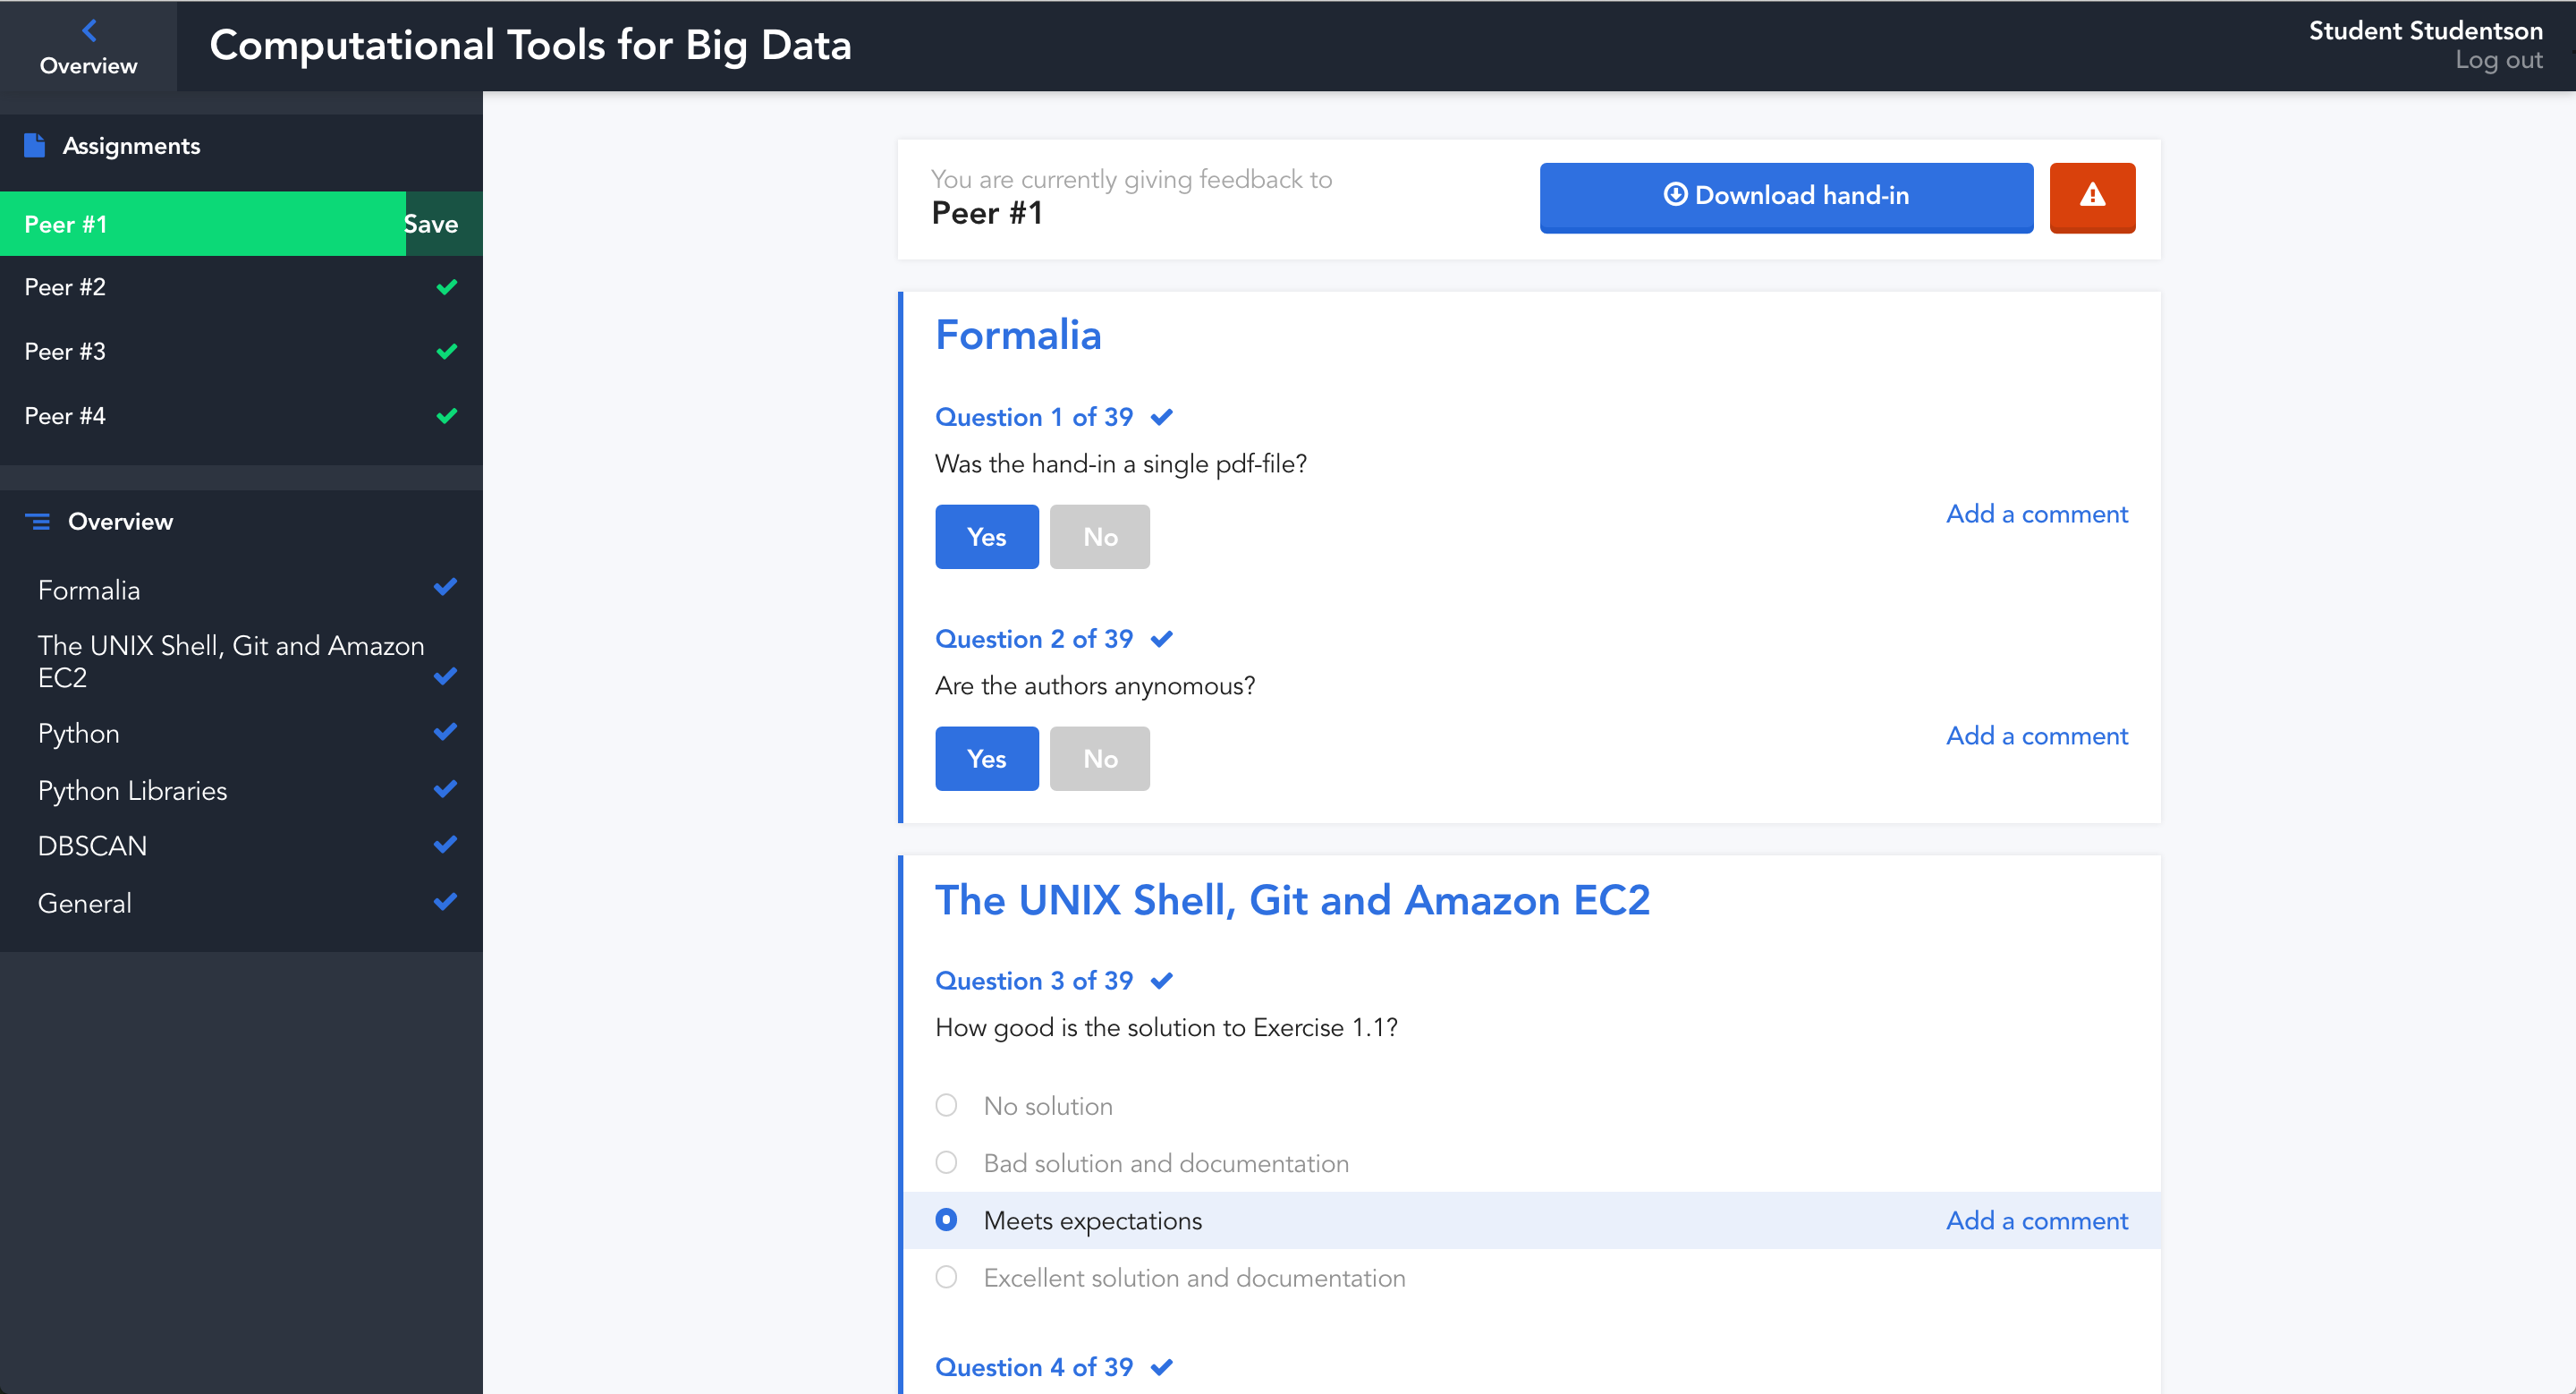
\includegraphics[width=\textwidth]{figures/screenshots/student_give_feedback.png}
  \caption[Screenshot from Peergrade.io]{A student grades another student's hand-in.}
  \label{fig:student-screenshot}
\end{figure*}

The last part of the platform is a complete overview of the assignment presented to the teacher with hand-ins, feedback, grades, constructive scores, statistical analysis for assignments, and statistical analysis of all the data to help the teachers give grades to the students. Furthermore the teacher is able to get a ``summary'' for a student to help grade the individual student and see how the students perform compared to other students. Figure~\ref{fig:teacher-screenshot} show screenshots of some of the interfaces seen by the teacher.

\begin{figure*}[ht!]
  \centering
  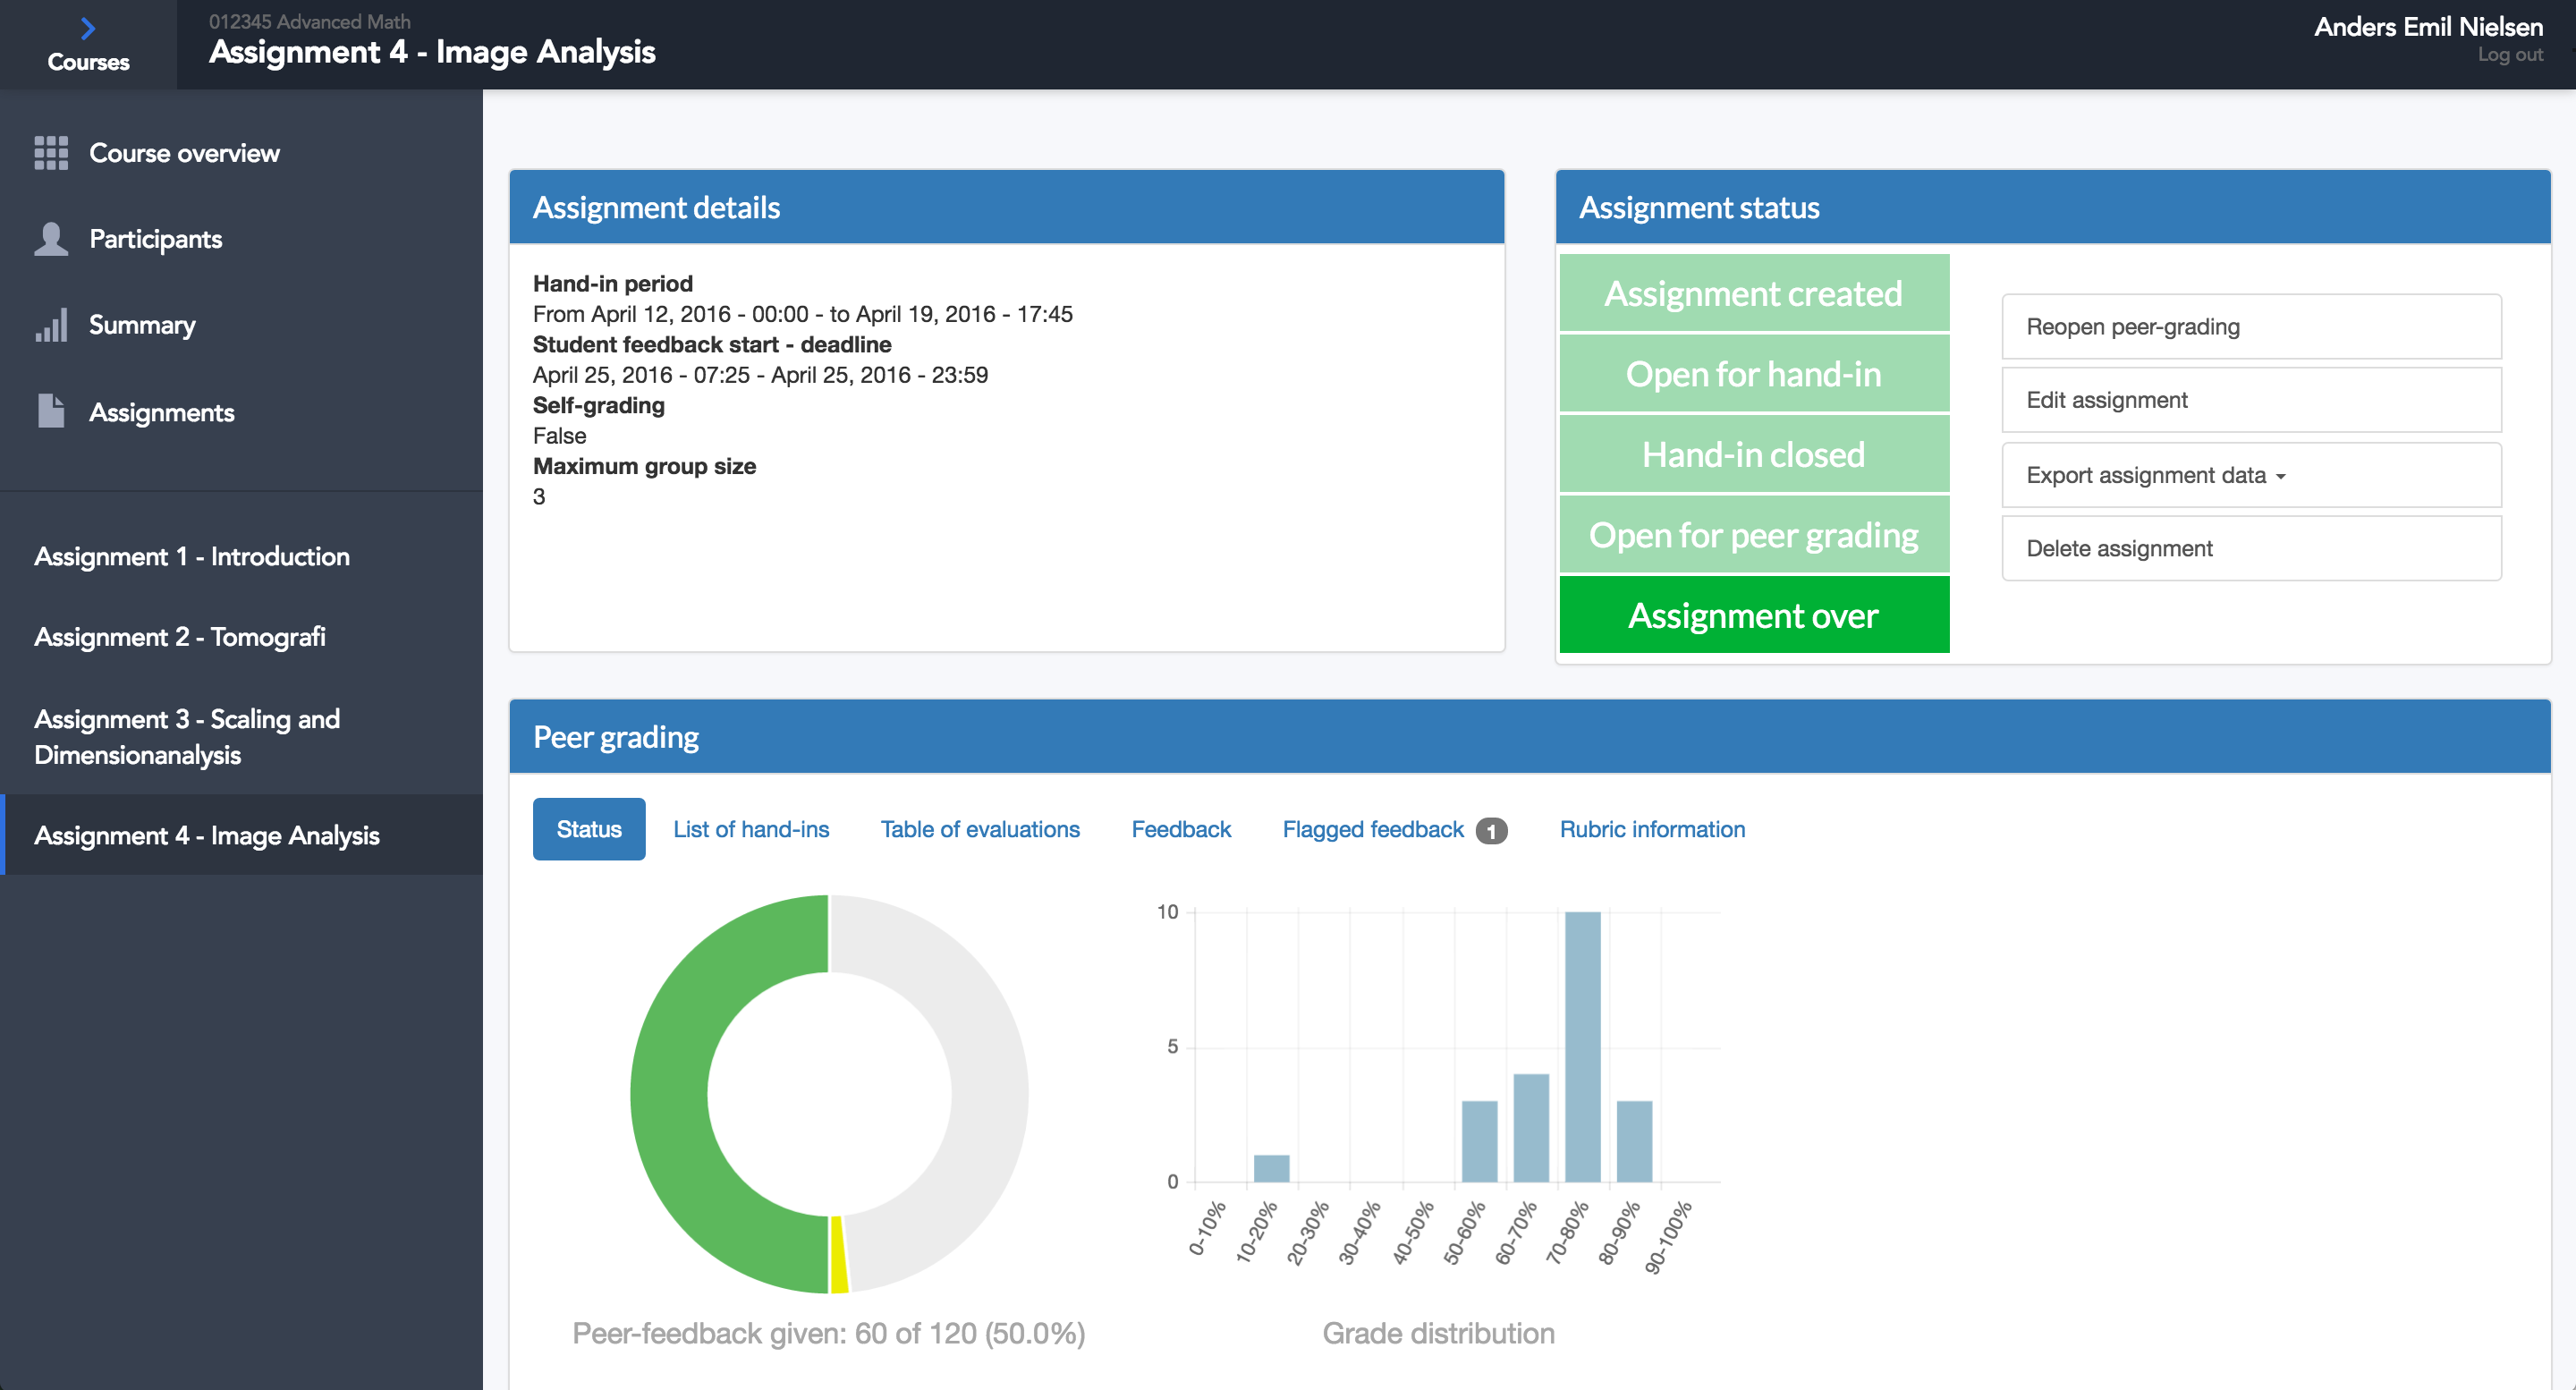
\includegraphics[width=1.0\linewidth]{figures/screenshots/teacher_assignment_overview.png}
  \caption[Screenshot from Peergrade.io]{A teacher sees the overview of a given assignment.}
  \label{fig:teacher-screenshot}
\end{figure*}

% subsection the-peergrade-io-platform end


\subsection{Running Example}
\label{subsec:running-example}

To relate the solution to a practical example, the thesis will use the running example seen in code snippet~\ref{code:running-example}.

\begin{code}{Code with the running example written in Python}
	\input{code/running_example.py}
	\label{code:running-example}
\end{code}

In this example we have a function \verb$course_score$ that computes the average score in a given course by fetching the participants from the primary data store and through iterations of each participant calculate the average score using the function \verb$participant_score$ that calculates the score of a single participant using a long running external method.

% subsection running-example end

% section context end

\section{Contributions}
\label{sec:contributions}

From the goal of finding and implementing a caching system that solves the problem in the context of the requirements described above, the thesis makes the following contributions.

First, research covering existing caching approaches for web development. We present a set of criteria used to evaluate caching approaches. These criteria are applied to existing approaches used in practical web development and proposed in research. The existing approaches are compared through an overview, which can be used to find a caching approach suitable for a given use case. By the end of the thesis the overview is extended with the solution proposed by this thesis, Smache.

Secondly, we present the design of Smache, a caching solution that aims to be easy to integrate into existing application and be able to cache the existing functions while invalidating and updating related cached values automatically. From this solution, the thesis makes the following technical contributions:

\begin{itemize}
  \item a \emph{programming model} that allows programmers to cache existing functions by declaring the dependencies to underlying data, after which the caching system automatically caches the result of the function by naming, localizing and storing the cached value for the function.
  \item a \emph{description and proof} of how to use \emph{timestamp invalidation} to invalidate and update cached values in a concurrent environment.
  \item an \emph{automatic invalidation system} based on \emph{timestamp invalidation}, a \emph{data structure} for representing dependencies between cached values and underlying data.
  \item a \emph{data update propagation algorithm} based on timestamp invalidation that is able to update all cached functions concurrently without additional concurrency control mechanisms.
\end{itemize}

Thirdly, we also present an implementation of Smache using the programming language Python, MongoDB as primary storage and Redis as the cache database, which is available open-source for future contributions at:

\url{https://github.com/anderslime/smache}

We have evaluated the performance and scalability of the data update propagation algorithm and how Smache affects existing operations on the application.

\section{Outline}
\label{sec:outline}

This thesis is structured as following:

With the motivation, problem, and requirements described in this introductory chapter, chapter~\ref{chapter:caching-model} will give an introduction to the basics of caching and present the models used and a set of criteria used to evaluate caching approaches.

The following chapter~\ref{chapter:caching} will describe the existing caching approaches described in literature and used in practice.

Based on the knowledge of existing solution, chapter~\ref{chapter:smache-cachable-functions},~\ref{chapter:invalidation}, and~\ref{chapter:data-update-propagation} describes the solution suggested by this thesis. The solution is explained using the programming model in chapter~\ref{chapter:smache-cachable-functions}. This model is then extended with automatic invalidation in chapter~\ref{chapter:invalidation} and afterwards with in-place updates in chapter~\ref{chapter:data-update-propagation}.

The solution is then evaluated and discussed based on test results and the initial requirements in chapter~\ref{chapter:evaluation}.

Chapter~\ref{chapter:caching-model} introduces caching by presenting the basic caching algorithm, the common architecture of caching system, the models used to describe caching approaches, and criteria used to evaluate caching approaches to find the appropriate technique.

Chapter~\ref{chapter:caching} will describe existing caching approaches with relation to caching evaluation criteria and explain how to choose a caching technique based on these criteria.

Chapter~\ref{chapter:smache-cachable-functions} presents the solution suggested by this thesis for the given context and requirements. First the techniques of existing approaches are discussed and followed by a description of the programming model - cachable functions.

Chapter~\ref{chapter:invalidation} describes in more details how the cachable functions are extended to have automatic invalidations using declared dependencies to underlying data.

Chapter~\ref{chapter:data-update-propagation} explains the data update propagation algorithm used to extend the cachable functions to have in-place cache updates.

Chapter~\ref{chapter:evaluation} goes through the test results related to performance, efficiency, and cache memory usages. The solution are then discussed and evaluated based on the test results and the initial requirements.

Chapter~\ref{chapter:conclusion} finalize the thesis with a conclusion.

% section outline end


% section contributions end

